\section{Preface}
\textit{The following chapter is the development of a pilot study of the suitability of Neural Field Theories for modelling time-varying activity in the context of topography I conducted at the University of Western Australia under the supervision Michael Small and Jennifer Rodger. The work in this chapter has been published in the paper \textbf{Development of Topographic Maps in Neural Field Theory with Short Time Scale Dependent Plasticity \cite{Gale2022-kq}}. This chapter focuses on mathematical analysis and adaption of the model into a pipeline whereby mouse (and other biological systems) data can be analysed and the efficacy of the model can be rigorously examined under Bayesian statistical frameworks.}

\section{Introduction}
Correlated neural activity has long been proposed as a driver of the development of topographic maps and now enjoys experimental support with the measurement of spontaneously generated waves of neural activity in the mammalian retina \cite{Chung1974-oy, Meister1991-mu, Ackman2012-uu, McLaughlin2003-yy, Stafford2009}. Disruptions to the patterning of these waves have been explored by knocking out the nicotinic-acetylcholine receptor subunit $\beta2$ which generates fast-spreading waves and thus a hyper-correlation -- where neurons are correlated at a far greater inter-neuron distance than in wild type -- between any two given retinal cells \cite{Stafford2009}. The effect of the $\beta2$ knock-out is to reduce the precision of the resulting topographic map: the receptive field of a given SC location is large with respect to wild-type \cite{Mrsic-Flogel2005-xp, McLaughlin2003-yy, Chandrasekaran2005-ug}. The current dogma of topographic mapping, as discussed in Section \ref{section:developmentaltheory} is that chemotactic signals drive the initial establishment of topography while the spontaneous activity patterns drive refinement to a required map precision.

The role of neural activity in a theoretical capacity is largely understood through the Hebb rule: correlated neural activity between two neurons strengthens the connection strengths between those neurons \cite{Hebb1949-wr}. This has been manifest in two ways: incorporating correlation profiles of activity between neurones, or modelling activity directly. Models that use correlation profiles typically include an isotropic spatial distance-dependent correlation which has been observed in mice, implicitly assuming that the correlation between retinal or colliculus firing rates decays exponentially in the distance between them \cite{Hjorth2015-le, Triplett2011-jk, Stafford2009}. These models by construction are unable to capture the various spatio-temporal statistics of the retinal waves condensing them all into a single correlation measure as a function of SC-distance. Modelling neuronal activity directly offers more flexibility in this regard but to proceed these models are usually evolved to their steady state after a presentation of a spatially oriented input stimulus and the nodes are given a binary classification of active/inactive on which the Hebb rule is applied  \cite{Willshaw1976-ew, Kohonen1982-nd, Stevens2013-ly, Takeuchi1979-zy, Detorakis2012-eh}. These models implicitly assume all transient neuronal information (such as spatio-temporally patterned stimulus waves) is averaged out. Recent efforts in a separate unified model which can incorporate dynamic activity were not able to quantitatively account for the $\beta2^{-/-}$ mutant data and are too computationally demanding for rigorous statistical analysis \cite{Godfrey2009-ts}. These considerations, as discussed in Section \ref{sec:beta2justification}, necessitate a deeper theoretical understanding of the spatio-temporal effects of neural activity in topographic map development.

The dense feed-forward connectivity pattern present in topographic systems make neural field theories (NFT) an attractive paradigm for modelling neural activity patterns in topographic systems. An NFT is a continuum model where the spiking activity of many neural inputs are averaged into a smoothly varying function over temporal and spatial locations. A theory of topographic development was proposed for an NFT which relied on static inputs in the pre-synaptic region resulting in activity patterns in the post-synaptic region stabilising to be time-independent and thus allowing a simple Hebbian plasticity rule to be applied \cite{Amari1977-gc}. The requirement for activity to stabilise before updating weights is also a feature of more general cortical map plasticity models \cite{Stevens2013-ly, Bednar2004-xl}. A more recent study used an NFT to model topography in the somatosensory cortex under thalamocortical plasticity using Oja's rule \cite{Detorakis2012-eh}. The assumption of static inputs limits the range of biological systems for which the theory developed in these works can apply in development. A candidate theoretical framework of Hebbian-based plasticity that can incorporate time-signatures of activity, spike timing dependent plasticity (STDP), has been developed for NFT \cite{Robinson2011-ve, Abbott2000-gl}; for a detailed discussion on this framework refer to Section \ref{sec:nftplsaticity}. The NFT modelling framework is continuous, rather than discrete, which allows for investigation of synaptic efficacy between locations rather than modelling individual synapses.

This chapter shall focus on developing the theory of activity by examining a simple NFT model equipped with an STDP based plasticity rule \cite{Amari1977-gc, Robinson2011-ve}. An asymptotic analytical solution will be developed for wave-like input stimuli. Markov-Chain-Monte-Carlo (MCMC) will be used to estimate the parameters that most adequately explain topographic refinement in both wild-type and $\beta2^{-/-}$ mice. Additionally, this analysis will provide a prediction about the time-scale on which the proposed plasticity operates. A glossary of symbols that will be used throughout the chapter is shown in Table \ref{table:glossary}.

\begin{table}
	\centering
	\begin{tabular}{| l || l |}
		\hline
		Symbol & Description \\
		\hline
		$S$ &Feed-forward kernel: pre-to-post regions \\
		$W$ &Recurrent kernel: post-to-post region \\
		$H$ &Synaptic evolution by spike-time envelope \\
		$Q$ &Map of membrane potential to spike-rate\\
		$u/U$ &Post-synaptic membrane potential/rates\\
		$a/A$ &Pre-synaptic membrane potential/rates\\
		$h$ &Form of activity waves\\
		$\Theta$ &Heaviside Theta function\\
		$\delta$ &Dirac-Delta distribution\\
		$\eta$ &Representation of white noise\\
		\hline
	\end{tabular}
	\caption{Symbols which are used to represent biological objects and/or processes. The parameters which are used to specify each functional form are omitted and detailed in later sections. \label{table:glossary}}
\end{table}

\section{Model}
A simple model architecture is chosen to closely imitate the system of interest: input from a continuous pre-synaptic field of nerve cells stimulates activity in a continuous post-synaptic field of nerve cells via a collection of feed-forward connections. These feed-forward connections will evolve under a plasticity rule governed by the spatio-temporal relations between the input and induced activity in the pre-synaptic and post-synaptic fields respectively. The activity in the post-synaptic field will be supported by inhibitory and excitatory sets of isotropic recurrent (or lateral) connections which, for simplicity, are static by assumption; for a description of non-isotropic recurrent kernels refer to \cite{Graben2014-pm, Schwappach2015-jy}. Changes in the feed-forward connections are dictated by firing activity in the pre-synaptic and post-synaptic fields. The activity dynamics in the post-synaptic field will be modelled by a neural field equation which couples a membrane potential and firing activity spatio-temporally. The pre-synaptic field activity could be modelled the same way but because there is no feed-back from the post-synaptic field it is sufficient to simply instantiate it which can be motivated by experimental spiking data \cite{Meister1991-mu}. The model architecture is summarised in Figure \ref{model-summary} and will now be explicitly detailed.
\begin{figure}[h!]
	\centering
	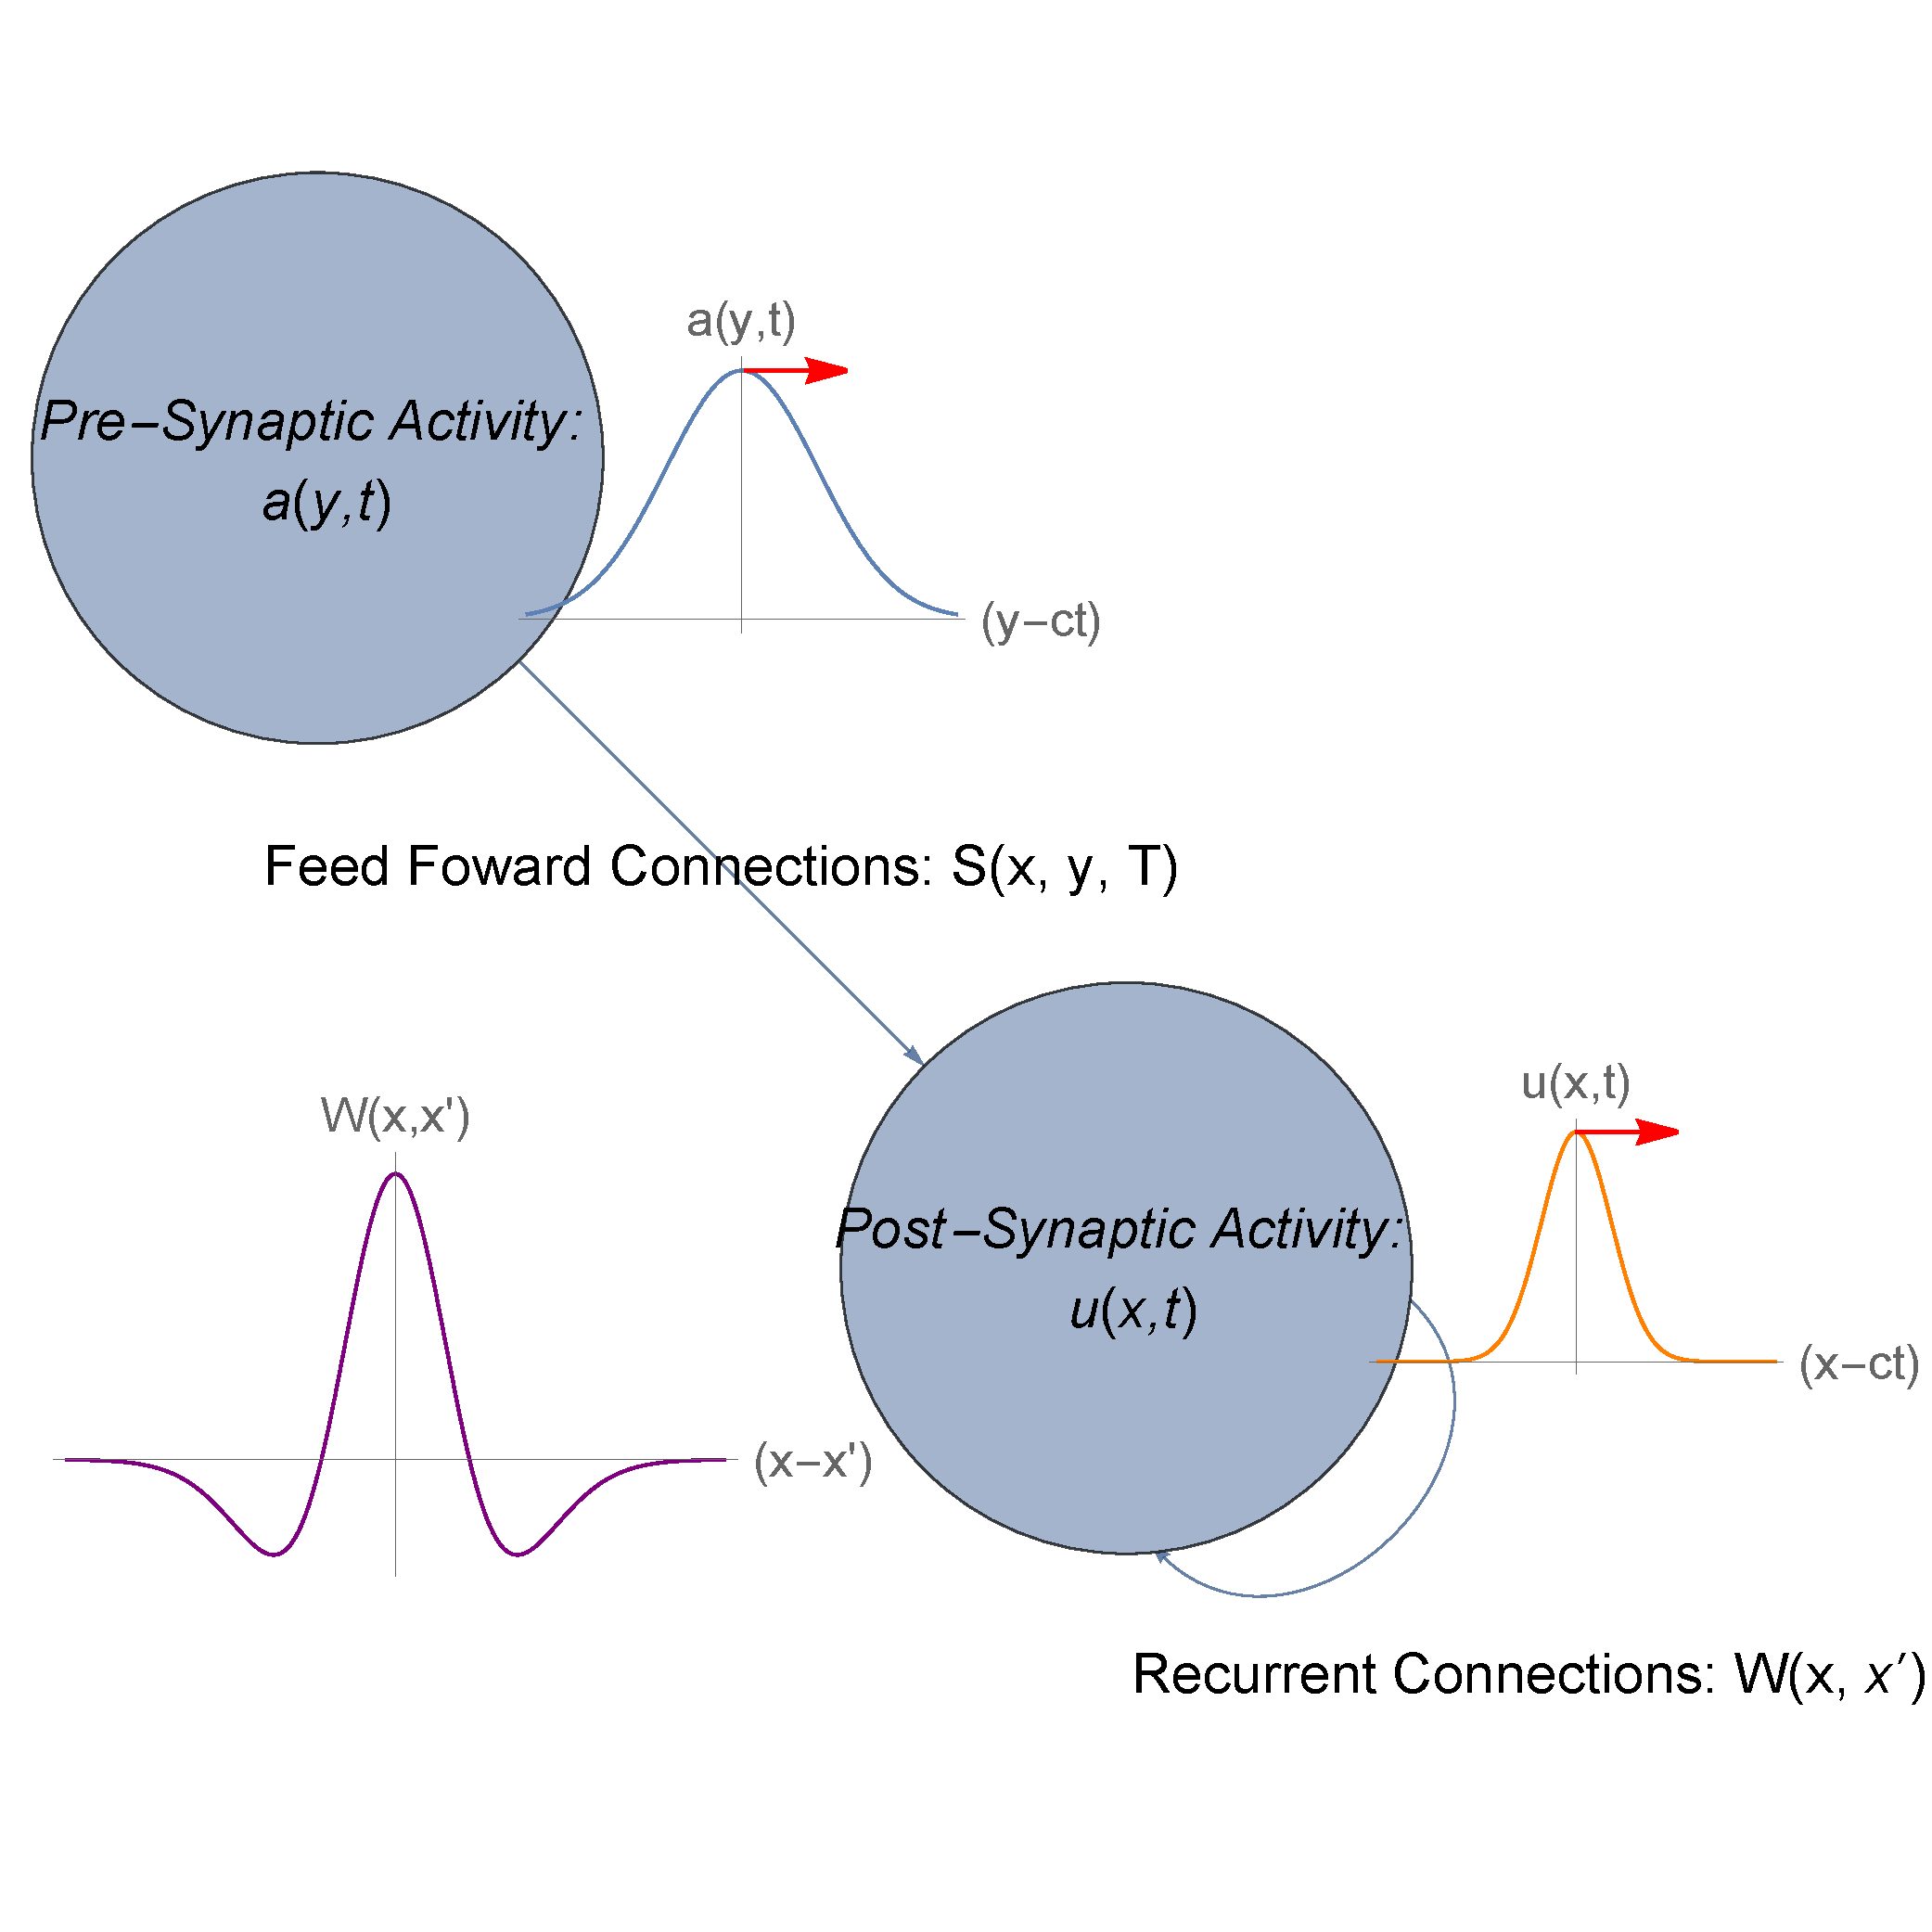
\includegraphics[width=0.7\textwidth]{images/nft_activity/model_summary}
	\def\c{The connections and directionality of the model: activity is fed-forward from the pre-synaptic region by the structure of interest and is spatial-temporally propagated by a time-differential operator and spatial convolution of inhibitory and excitatory recurrent connections. }
	\caption[\c]{\c Cartoons of typical propagating activity patterns and recurrent connections are shown but not feed-forward connections as determining these are the object of this study. The generated signal in the post-synaptic region and the driving signal in the pre-synaptic region are then convolved with a plasticity window to inform the synaptic changes on a slow time scale which is indicated by the variable $T = \epsilon t$ for some small $\epsilon$. \label{model-summary}}
\end{figure}
\paragraph{Representation of Topography}
What topography means in the continuous sense should be established. Two things should be preserved: the neighbourhood projection, and the excitatory feed-forward nature of the network. To preserve the neighbour-neighbour relation the connections, here referred to as a synaptic distribution, labelled $S$, and measured in synapses per mm$^2$,  should take the form:
\begin{equation}
	S(x,y,T) = S(|x-p(y)- \rho|, T),
\end{equation}
where $p(y)$ is some monotonically increasing function and $\rho$ is some constant to indicate that a coordinate shift still permits a topographic mapping. The excitatory feed-forward nature means that a patch of activation in the pre-synaptic field should activate a local patch of the post-synaptic field associated with its topographically projected location. Therefore, $S$ should decay quickly at infinity, be positive at the topographically projected location, and have a finite (small) radius at which it transitions to being negative. Alternatively, it can be strictly positive but quickly decaying such that it never over-powers the recurrent inhibitory connections; see Figure \ref{fig:topographicexamples}.

\begin{figure}[h!]
	\begin{subfigure}{0.4\textwidth}
		\centering
		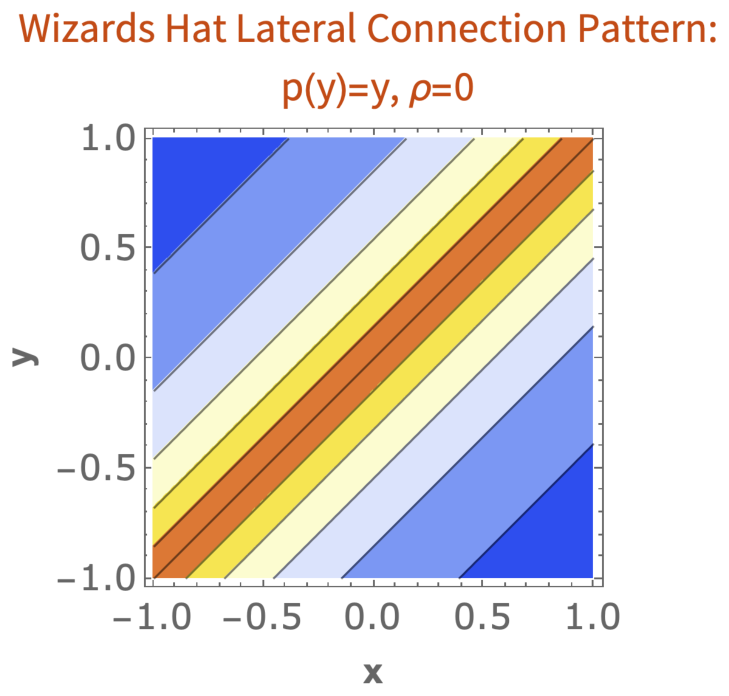
\includegraphics[width=\textwidth]{images/nft_activity/example-topographicorganisationlinear}
		\caption{}
	\end{subfigure}
	\begin{subfigure}{0.52\textwidth}
		\centering
		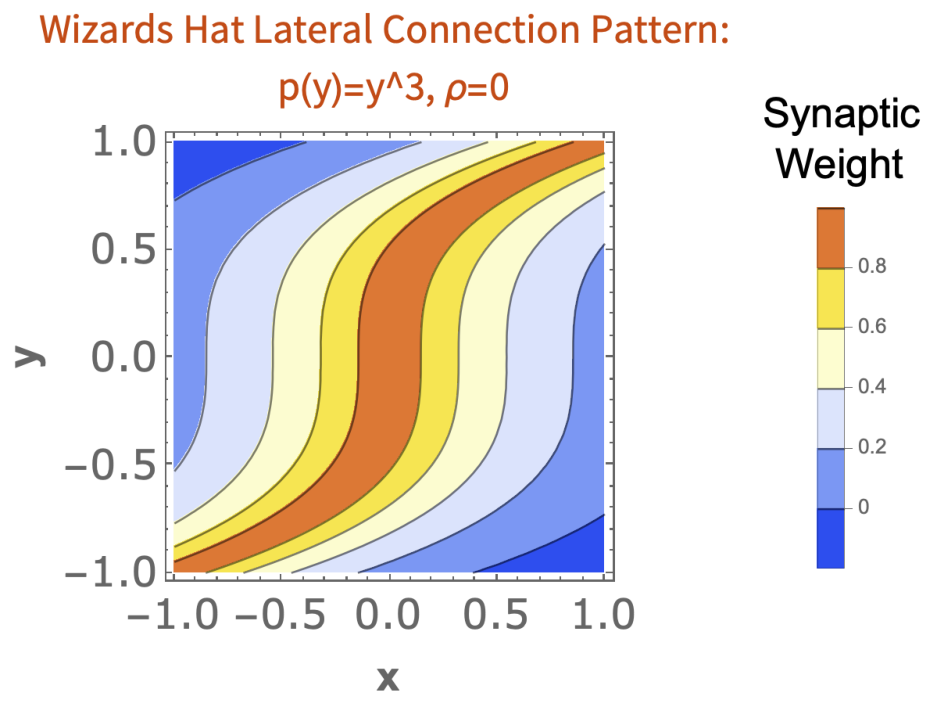
\includegraphics[width=\textwidth]{images/nft_activity/example-topgographicorganisationcubic}
		\caption{}
	\end{subfigure}
	\def\c{Two examples of topographic organisation using a Wizard hat style function: a) shows a linear relationship between axes and for while b) shows a cubic relationship between axes. }
	\caption[\c]{\label{fig:topographicexamples}  \c Both are topographic but a) has an even representation of the pre-synaptic field across the post-synaptic field while b) compresses the representation at the boundary and enlarges the interior.}
\end{figure}
\paragraph{Neural Field Theory}
The model is formed using NFT formulation proposed by Amari (1970) which considers both excitatory and inhibitory connections in the same kernel $W$ \cite{Amari1977-gc}. The pre-synaptic and post-synaptic regions are coupled by a kernel $S$. It is this kernel in which the evolution of topography is demonstrated. The electrical activity, measured in millivolts (mV), of the pre-synaptic field is denoted by $a(x,t)$ and in the post-synaptic field by $u(x,t)$, and choose the firing rate function to be a sigmoid-logistic function:
\begin{equation}
	Q(u)=\frac{Q_\text{max}}{1+\exp(-\beta(u-\theta))},
\end{equation} 
where $\beta$ and $\theta$ dictate the steepness of the curve and the threshold respectively, and $Q_{\text{max}}$ is the maximal firing rate; { the units of each are mV$^{-1}$, mV, and spikes per second and can be found in Table \ref{table:parameters}}. The activity dynamics are then governed by the internal dynamics mediated by $W$ and the input provided through the pre-synaptic field, $Q(a)$, and its transfer through $S$:
\begin{align}
	\begin{split}
		u(x,t)&
		+\tau \frac{\partial u(x,t)}{\partial t} 
		- \int_{-\infty}^{\infty} W(x, x^\prime) Q(u(x^\prime,t)) dx^\prime = \int_{-\infty}^{\infty}S(x,y, T) Q(a(y,t)) dy.
	\end{split}
	\label{eq:amari}
\end{align}
Note that the time variable $T$ is on a much slower time scale which is realised by setting $t=\epsilon T$ for $0<\epsilon \ll 1$. For the purposes of solving equation \ref{eq:amari} these connections can be considered effectively constant. A simplifying assumption is that the recurrent connections $W$ remain constant throughout the course of synaptic development and are homogenous. Following Robinson (2011) a plasticity window is defined as a rapidly decaying envelope $H$ that weights the cross-correlation of the input and response signals in a population in the same fashion as biologically-inspired plasticity rules weight individual spikes of a neuron \cite{Robinson2011-ve}. { These plasticity windows have been observed in several organisms and brain regions; a typical window has a time constant on the order of 10s of milliseconds but have been observed to be on the order of 10s of minutes \cite{Froemke2002-be, Zhang2000-lb, Allen2003-rw, Markram1997-ln, Citri2008-kv}}. The average synaptic dynamics are given by averaging over a time-window which is longer than the time-scale of the plasticity window and of the inverse frequencies of the forcing and the response stimuli but shorter than any long term plasticity changes:
\begin{align}
	\tau'\frac{dS(x,y,T)}{dT} = \int_{-\infty}^{\infty} \langle U(x,T+s)H(s)A(y,s) \rangle ds, \label{eq:robinson}
\end{align}
where $U=Q(u), A=Q(a)$ (the firing rates of the post-synaptic and pre-synaptic populations respectively), $\langle \cdot \rangle$ denotes averaging, and $\tau^\prime$ is the time-scale of synaptic dynamics. In the case of no electrical activity present in the pre-synaptic field there will be a constant level of spontaneous firing $A$ inducing an electrical activity and firing rate $U$ which in turn will lead to run-away synaptic dynamics. The dynamics of the average rate of synaptic change and the expected synaptic values are of key interest; in later sections this will be taken as an adiabatic expansion and averaging over stimulus input locations. Therefore, the above equation should include a noise term $\eta$ with strength $\kappa$ to incorporate the small deviations of spontaneous activity:
\begin{align}
	\tau^\prime\frac{dS(x,y,T)}{dT} = \int_{-\infty}^{\infty} \langle U(x,T+s)H(s)A(y,s) \rangle ds + \kappa\eta(x,y,t).
\end{align}
\paragraph{Regularisation}
Several regularisation rules have been posed to stabilise these unstable Hebbian dynamics and are broadly classified in the form of subtractive and multiplicative rules \cite{Abbott2000-gl}. A subtractive normalisation rule is chosen to stabilise the dynamics, assuming there is some atrophic factor to regulate the unbounded growth of synapses, governed by parameter $\lambda$, released at each location:
\begin{align}
	\begin{split}
		\tau^\prime&\frac{dS(x,y,T)}{dT} + \lambda S(x,y,T)=  \int_{-\infty}^{\infty} \langle U(x,T+s)H(s)A(y,s) \rangle ds + \kappa\eta(x,y,t).
	\end{split}
	\label{eq:stdpfinal}
\end{align}
The idea of a synaptic decay on the basis of metabolic demands has also been introduced in a study of organisational behaviour in V1 \cite{Wright2013-td}. The dynamics of equation \ref{eq:stdpfinal} are focused on for the remainder of this text.
\paragraph{Perturbations}
The post-synaptic field is assumed to relax in the absence of forcing activity that i.e. there is a constant level of spontaneous firing in the pre-synaptic and post-synaptic fields; note that this is not necessarily the case \cite{Coombes2005-mt}. All activity dynamics are assumed to be small perturbations from these constant rates. Furthermore, if one makes the assumption that the firing rates can be expressed as perturbations from a baseline firing rate,  $U(x,t) = U_0 + \delta U(x,t)$ and $A(x,t) = A_0 + \delta A(x,t)$, then taking Fourier transforms the average change in plasticity in the un-regularised dynamics can be expressed as:
\begin{equation}
	\frac{1}{2\pi}  \int_{-\infty}^{\infty} \delta \hat{U}(x,\omega) \hat{H}(\omega)^* \delta\hat{A}(y,\omega)^*d\omega,
\end{equation}
where $\hat{\cdot}$ denotes the Fourier transform, and $\cdot^*$ denotes complex conjugation \cite{Robinson2011-ve}. 

\paragraph{Input Stimulus}
Two classes of input stimulus are considered: mono-directional and bi-directional (radial) waves. Mono-directional waves propagate either to the left/right at speed $c$ starting at some time $t_0$ and some starting position $y_0$ finally finishing at some time $t_1$. These terms are rooted in a two dimensional consideration of the problem. A mono-directional wave might travel along a single radial angle whilst a radial wave travels isotropically. { These choices allow for a description of the waves observed in the retina  \cite{Meister1991-mu, Stafford2009, Ackman2012-uu}. Of the two the mono-directional wave is the most appropriate model but the bidirectional wave is an equivalent but analytically preferable case as shown in Section \ref{sec:monotoradial}}. Letting $r(y,t)=y-ct-y_0$, these inputs accordingly take the form:
\begin{equation}
	a(y,t) = (\Theta(t-t_0)-\Theta(t-t_1))h(r(y,t)). \label{wave:plane}
\end{equation}
Radial inputs are similar, simply propagating in both directions:
\begin{align}
	a(y,t) = \frac{(\Theta(t-t_0)-\Theta(t-t_1))(h(r(y,t))+h(r(y,-t)))}{2}. 
	\label{wave:radial}.
\end{align}
In both cases $h$ is used to denote the shape of the propagating wave-form. The choice of $h$ is left to be general but can be thought of as a travelling Gaussian wave-packet. A function may be approximated by a linear sum of appropriately weighted Gaussian's and so this forms a basis set and the simple case is considered in Section \ref{sec:param}.
\paragraph{Plasticity Windows}
There are two general forms of plasticity considered: time symmetric and time asymmetric plasticity. Time symmetric plasticity, also called Correlation Dependent Plasticity (CDP), means that connections are strengthened by spikes that are separated by short times and weakened by medium-long time separated spikes, but in which the ordering of the spikes is not important. Time asymmetric plasticity, or STDP, means that not only does the temporal closeness of pre-synaptic and post-synaptic spikes matter but the ordering in which they occur: post-synaptic firing that occurs before pre-synaptic firing weakens the connection and vice-versa. A canonical form of these two rules expressed as a plasticity envelope is given by:
\begin{equation}
	H(s) = \begin{cases}
		A_+\exp(-\frac{s}{t_p}) \quad &s\geq 0\\
		A_-\exp(\frac{s}{t_p}) \quad &s <0
	\end{cases}
\end{equation}
where $A_-=A_+$ for CDP and $-A_-=A_+$ for STDP, and $t_p$ is the time-scale of the plasticity \cite{Abbott2000-gl}. The Fourier transforms of these learning rules are:
\begin{align}
	\hat{H}_{CDP}(\omega) &= \frac{2A_+}{1+\omega^2 t_p^2} \label{rule:CDP}\\
	\hat{H}_{STDP}(\omega) &= \frac{2A_+\omega it_p}{1+\omega^2 t_p^2} \label{rule:STDP}
\end{align}
In summary, a membrane signal is generated in the post-synaptic region on a fast-time scale which is supported by recurrent connections and generated by input from a pre-synaptic region. The spatial-temporal patterns of the pre-synaptic and post-synaptic activity then inform synaptic changes between the two regions on a slow time scale in accordance with a plasticity rule.

\section{Analysis}
The connectivity kernels, pre-synaptic stimuli, and post-synaptic activity and firing rates are assumed to be elements of Schwartz space i.e. the functions and derivatives that define these rates decay quickly at long range and they are localised. This assumption is made to ensure bio-physical realism. Connectivity kernels typically have short-range and long-range interactions but they do not interact at all with very distal connections and their functions must accordingly decay at infinity. Similarly, due to these recurrent connectivity kernels, electrical signals only seem to be able to support themselves on finite distances and they too must accordingly decay. The assumption of Schwartz functions ensures the Fourier transforms existence and makes formulating the problem in Fourier space desirable.

\paragraph{Approximating Input Stimulus}
The inputs specified earlier are biologically realistic but will become more tractable if one of the Heaviside functions can be removed; this would amount to a stimulus propagating to infinity after being initialized. This approximation can be made if the synaptic change induced by this different stimulus is arbitrarily small when compared to the synaptic change induced by the true stimulus. This is realised by the rapid decay of the plasticity window and shown formally in Lemma \ref{lemma:decay}; see Appendix A.

\paragraph{Activity Dynamics}
It was reasoned on physical grounds that in the absence of pre-synaptic stimulation the only post-synaptic solution is a static, constant level of activity. Synaptic dynamics are governed by perturbations from this baseline and expressions for these are derived in this section. The baseline is assumed to be sufficiently close to the origin that the logistic function is analytical and has a convergent Taylor series expanded around $u = u_0$. Therefore, a good approximation is:
\begin{equation}
	Q(u) = Q(u_0) + u Q'(u_0). \label{eq:firingapproximation}
\end{equation}
This can then be inserted in equation (\ref{eq:amari}) and a Fourier transform can be taken to yield:
\begin{align}
	\hat{u}(k,\omega) = Q&(u_0)\Gamma(k,\omega)(\hat{W}(k)+\hat{S}(k))\delta(k)\delta(\omega) + Q'(u_0)\hat{S}(k)\Gamma(k,\omega)\hat{a}(k,\omega),
\end{align}
where $\Gamma(k,\omega)=(1 + i\tau\omega - \hat{W}(k))^{-1}$. Now, recognising that $Q(u_0)\Gamma(\omega,k)(\hat{W}(k)+\hat{S}(k))\delta(k)\delta(\omega)$ corresponds to the static solution, i.e. the baseline activity level, the expression for the Fourier transform of the perturbation of the activity level is: 
\begin{equation}
	\delta\hat{U}(k,\omega) =\hat{S}(k)\Gamma(k,\omega)\hat{a}(k,\omega),
\end{equation}
where $U(x,t)=Q(u(x,t))$. The Fourier Transform of the perturbation from the baseline rate in the pre-synaptic field, $\delta A(y,t)$ is trivial to compute: $ \delta \hat{A}(k,\omega)=\delta \hat{a} (k,\omega)$. This is sufficient to explicitly compute the synaptic change between any two points in the pre-synaptic and post-synaptic field. 
\paragraph{Synaptic Dynamics}
The synaptic field, and synaptic changes are assumed to be isotropic; $S(x,y,T) = S(x-y,T)$ for all $T$. Then, making the approximation of the firing rate, and taking spatial Fourier transforms the synaptic change can be written:
\begin{equation}
	\delta(p+k)\frac{d\hat{S}(k,T)}{dT} = \delta(p+k)(S_0 - S_1 \hat{S}(k,T)) +  S_2\int_{-\infty}^{\infty}  \hat{a}(\omega,p)\hat{a}(\omega,k)^* \hat{H}(\omega)^* \hat{S}(k,T)^*\Gamma(\omega,k)  d\omega ,
\end{equation} 
where $S_0$, $S_1$, and $S_2$ have absorbed the time constant, regularisation constants, baseline firing rate, and the Fourier normalisation terms. The sign of $S_1$ is negative to indicate its relationship with the decay constant $\lambda$. Integrating with respect to $p$, the above equation may be solved as:
\begin{align}
	&\frac{d\hat{S}(k,T)}{dT} = S_0 - S_1\hat{S}(k,T) + S_2\hat{S}(k,T)^*\int_{-\infty}^{\infty}\mathcal{B}(\omega)\hat{a}(\omega,k) \hat{H}(\omega)^* \Gamma(\omega,k) d\omega,
\end{align}
where $\mathcal{B}(\omega) =  \int_{-\infty}^{\infty} \hat{a}(\omega,p)^*dp$. The connectivity kernel $S$ in position space is physically required to be real. This kernel is written as the composition of odd and even functions. Then, from conjugate symmetry it follows that its Fourier transform is composed of a real part consisting of the linear combination of the Fourier transforms of its even components, and an imaginary part consisting of the linear combination of the Fourier transforms of its odd components. For $S$ to remain real its derivative must have an even function as its real component, and an odd function as its imaginary component. Let,  
\begin{equation} 
	G(k)= \int_{-\infty}^{\infty} \left(\int_{-\infty}^{\infty}  \hat{a}(p,\omega)^*dp\right)\hat{a}(\omega,k) \hat{H}(\omega)^* \Gamma(k,\omega) d\omega.
\end{equation}
If $G(k)$ is even and real, or odd and purely imaginary, then the above equation can be separated into odd and even parts and solved as two independent ODEs. Attention will be restricted to the even form of $G(k)$ for reasons detailed in the following section. Denoting $S_{O}(x,T)$ and $S_E(x,T)$ to be the odd and even parts of the coupling function in position space these ODEs are then: 
\begin{align}
	&\frac{d\hat{S}_O(k,T)}{dT} =-(S_1 + S_2 G(k)) \hat{S}_O(k,T) \\
	&\frac{d\hat{S}_E(k,T)}{dT} = S_0 + (S_2 G(k) - S_1) \hat{S}_E(k,T) .
\end{align}
Therefore, in the asymptotic limit, provided $S_1 + S_2 G(k)>0$, the odd components of the initial organisation decay to zero and provided $S_1 > S_2 G(k)$ the even components have solution:
\begin{equation}
	\hat{S}_E(k) = \frac{S_0}{S_1 - S_2G(k)}. \label{eq:asymptoticsynapse}
\end{equation}
The final organisation is therefore dictated by the initial even components and the form of $G(k)$. $G(k) > 0$  is sufficient to satisfy the above conditions and this will be accordingly shown. The form of $G$ is prescribed by the learning rule employed and the input stimulus used and referred to as the training function.

\paragraph{Mono-Directional Propagation} \label{sec:monotoradial}
Supposing the input stimulus is $a(y,t) = \Theta(t) h(y-ct-y_0)$ it is fairly straightforward to show that the training function $G$ is not even and therefore will not work as a training function. However, assuming that the synaptic changes are adiabatic or reasonably small and assuming the proportions of waves propagating left and right are equal then the average synaptic dynamics induced by inputs of the mono-directional form (equation \ref{wave:plane}) are the same as the dynamics induced by inputs of the radial form (equation \ref{wave:radial}). Attention is therefore restricted to radially propagating inputs.
\paragraph{Radial Propagation}
Presume the input stimulus is in the form $a(y,t) = \Theta(t) (h(y-ct-y_0)+h(y+ct-y_0))$. Taking two Fourier transforms yields:
\begin{align} 
	\begin{split}
		\hat{a}(p,\omega)& = \frac{1}{2} e^{-2\pi i y_0 p}\hat{h}(p) \left( \delta (w+cp) + \delta (w-cp) + \frac{2iw}{\pi (w-cp)\pi (w+cp)}\right).
	\end{split}
\end{align}
Integrating with respect to $p$ by using the Cauchy Residue Theorem and evenness of the last term and $\hat{h}$ gives:
\begin{equation} 
	\label{integrateap}
	\int_{-\infty}^{\infty}\hat{a}(p,\omega)^*dp = \left(1 + \frac{2}{c} \right) \hat{h}\left(\frac{\omega}{c}\right)^* \cosh\left(2\pi i y_0 \frac{\omega}{c}\right).
\end{equation}
$G(k)=G(k; y_0)$, assuming the synaptic changes at each time step are small, the average synaptic change can be written as:
\begin{equation}
	\left \langle \frac{d\hat{S}(k,T)}{dT} \right \rangle = S_0 - S_1\hat{S}(k,T) + S_2 \hat{S}(k,T) \langle G(k; y_0, c) \rangle. 
\end{equation}
The asymptotic limit, which is the target of this work, will approach this average and for the remainder of this work angle brackets are dropped. Let $g(k;c) = (\hat{H}(ck)^* \Gamma(k,ck)+\hat{H}(-ck)^* \Gamma(k,-ck))/c$. Equation (\ref{integrateap}) can then be inserted into the expression for $G(k)$ and the Dirac-Deltas can be integrated. Then, $y_0$ is integrated out by assuming it is distributed over some interval of length $L$ giving exponential integral functions which vanish as $y_0 \rightarrow \infty$ yielding:
\begin{equation}
	\frac{d\hat{S}(k,T)}{dT} = S_0 + \hat{S}(k,T)\left(S_2 g(k;c) |\hat{h}(k)|^2 - S_1 \right), \label{eq:finalsyn} 
\end{equation}
Showing that $g(k;c)$ is even may be done by direct substitution for both STDP and CDP rules under the assumption that both $W$ and $h$ are even. It follows that all $G(k)$ are even. It remains to be shown that $G(k)$ is restricted to being non-negative or non-positive. All the scaling constants are positive and it is therefore clear for the STDP rule that $G(k)\geq 0$, while for the CDP rule $G(k)$ is never non-positive and is only non-negative if $\hat{W}(k)<1$. It is certainly possible that this is the case, but it is not true for common choices of $W$. $W$ is typically chosen to be in the form of a ``wizard-hat" with short-range excitation and long range inhibition which is theoretically grounded and observed experimentally \cite{Sirosh1994-zv, Phongphanphanee2014-in}.
\subsection{Computational Analysis and Parameter Estimation}
There has been little reference to the recurrent connections or input stimulus (with the exception of wave-speed $c$) and the parameters and functional forms that characterise them. These will now be explicitly defined and the consequences of this choice examined by computational means. Key parameters of the model contributing to width (arbor size) will be estimated by means of Markov Chain Monte Carlo (MCMC) applied to wild-type and $\beta2^{-/-}$ mutant data. This estimation allows for both model validation and estimation of biological quantities which have not yet been experimentally examined.

The wave-form of the input stimulus is modelled as a Gaussian with amplitude and width (variance) parameters of $\sigma_1$ and $\sigma_2$ respectively and with Fourier Transform $\hat{h}(k) = \sigma_1 \sigma_2\exp(-k^2\sigma_2^2/2)$. The recurrent connections are described by a difference of two Gaussians: $\hat{W}(k) =  r_1\exp(-k^2 r_1^2/2) -  R_1r_2\exp(-k^2 r^2)$. This choice ensures that the dimensional requirements for the propagator are satisfied and that $|W(k)|<1$ for a suitable choice of recurrent connection parameters. These choices mean that there are 16 key biological parameters: $u_0, \tau, \tau^\prime, \kappa, \lambda, A_p, t_p, Q_\text{max}, \beta, \theta, $\\$c, \sigma_1, \sigma_2, R_1, r_1, r_2$.

\paragraph{Parameter Analysis} \label{sec:param}
Examination of equation \ref{eq:asymptoticsynapse} shows that $S_0$ (or $\kappa/\tau^{\prime})$ serves to stabilise the dynamics at the cost of introducing noise - the Fourier spectrum of a biologically realistic organisation will decay to a constant i.e. to a baseline level of white noise. A tolerable level of system noise is expected and it is assumed that this noise can be filtered by some means. The denominator dictates the deviations from this noise and noting that for both CDP and STDP $G(k) \rightarrow 0$ and $G(k)>0$ ensures that physically viable solutions enforce $0<G(k)<S_1/S_2$ and non-viable solutions contain pairs of singularities (via evenness of $G$) where $G(k)>S_1/S_2$ for some $k$. 

An arbitrarily large wave-amplitude $\sigma_1$ can force a singularity in both cases and an arbitrarily large $c$ can force a singularity in the STDP case. Therefore, stability in the STDP case that the maximum wave speed is bound by a contour inversely proportional to wave-amplitude and vice-versa. Given the likely biological restrictions on amplitude this implies that wave speed could be dictated in part by wave amplitude. With this in mind $\sigma_1$ is set to $5$mV for the remainder of this work. This ensures that there is a baseline distinguishable level of firing when the wave reaches its peak amplitude but the neurons are not near a saturated level thus satisfying the assumptions required for the approximation in equation \ref{eq:firingapproximation}. The parameters $u_0, \tau^\prime, \lambda, A_p, f_\text{max}, \beta, \theta$ are absorbed into $S_0, S_1$, and $S_2$ and their effects on the dynamics are immediate: they dictate the absolute measurable values of the organisation, not the form. These parameters are set according to Table \ref{table:params} for the remainder of this work.

\begin{table}[h!]
	\centering
	\begin{tabular}[width=0.5\textwidth]{| l || l | l | l |}
		\hline
		Param. & Value & Units  & Description \\
		\hline
		$u_0$ & -58 & mV & Resting potential \\
		$\tau$  & 0.1 & s & Activity time-scale \\
		$\tau^\prime$  & 100 & s & Synaptic time-scale \\
		$\kappa $  & 0.001 & syn.mm$^{-1}$ & Synapse density \\
		$\lambda $  & 0.001 & $-$ & Decay rate\\
		$A_p $  & 1 & syn.mm$^{-1}$  s & Hebbian rate\\
		$t_p $  & 1.0 & s  & Hebbian time-scale\\
		$Q_\text{max} $  & 1 & s$^{-1}$   & Max firing rate\\
		$\beta$ & 0.26 & mV$^{-1}$ & Rate steepness\\
		$\theta$ & -45 & mV & Rate threshold\\
		$c$ & 0.1 & mm s$^{-1}$ & Wave-speed\\
		$\sigma_1$ & 5 & mV & Wave-amplitude\\
		$\sigma_2$ & 0.1 & mm & Wave-length\\
		$R_1$ & 1.08 & syn.mm$^{-1}$ &Recurrent amplitude\\
		$r_1$ & 0.129 & mm &Inhibitory length-scale\\
		$r_2$ & 0.136 & mm &Excitatory length-scale\\
		\hline
	\end{tabular}
	\def\c{Choices for the biological parameters used in a neural field theory model of topographic development. }
	\caption[\c]{\label{table:params} The choices made for each of the biological parameters used throughout the chapter, unless otherwise stated. The length scale is chosen to reflect the scale at which NFT typically applies in the brain and the appropriate scale for the mouse SC \cite{Robinson2005-en}. The resting membrane potential, the threshold voltage, and the voltage scale are estimated to be in line with electrophysiological recordings \cite{Shi2018-er}. These parameters should be carefully measured if a specific biological system is to be closely analysed. \label{table:parameters}}
\end{table}

CDP $G(k)$ attains its global maximum at $k=0$ meaning that its stability is determined entirely by the relationship between $S_1$ and $S_2$. Furthermore, with CDP synaptic changes have the potential to be overly large with no parameter available to mitigate them. In the STDP case the small timescale ensures that the changes are small and the adiabatic assumption is satisfied. Attention is now restricted to the STDP case noting that extending the analysis to a CDP rule would be straightforward but care must be taken in the choice of parameters.

These choices, while considered, have reduced the problem to a single learning rule and several key parameters. It should be stressed that the other parameters must be carefully measured for accurate predictions and are in some sense non-trivial: one can manipulate them biologically and cause a bifurcation in the organisation dynamics. Figure \ref{fig:stablity} demonstrates the manifold in the $c-\sigma_2$ plane for which the model presents plausible (stable) solutions. Only a 2-dimensional slice of the overall manifold for which there are no solutions with singularities is shown, but care should be taken in ensuring that any solution of interest lies within the volume of this manifold for all parameters.
\begin{figure}
	\centering
	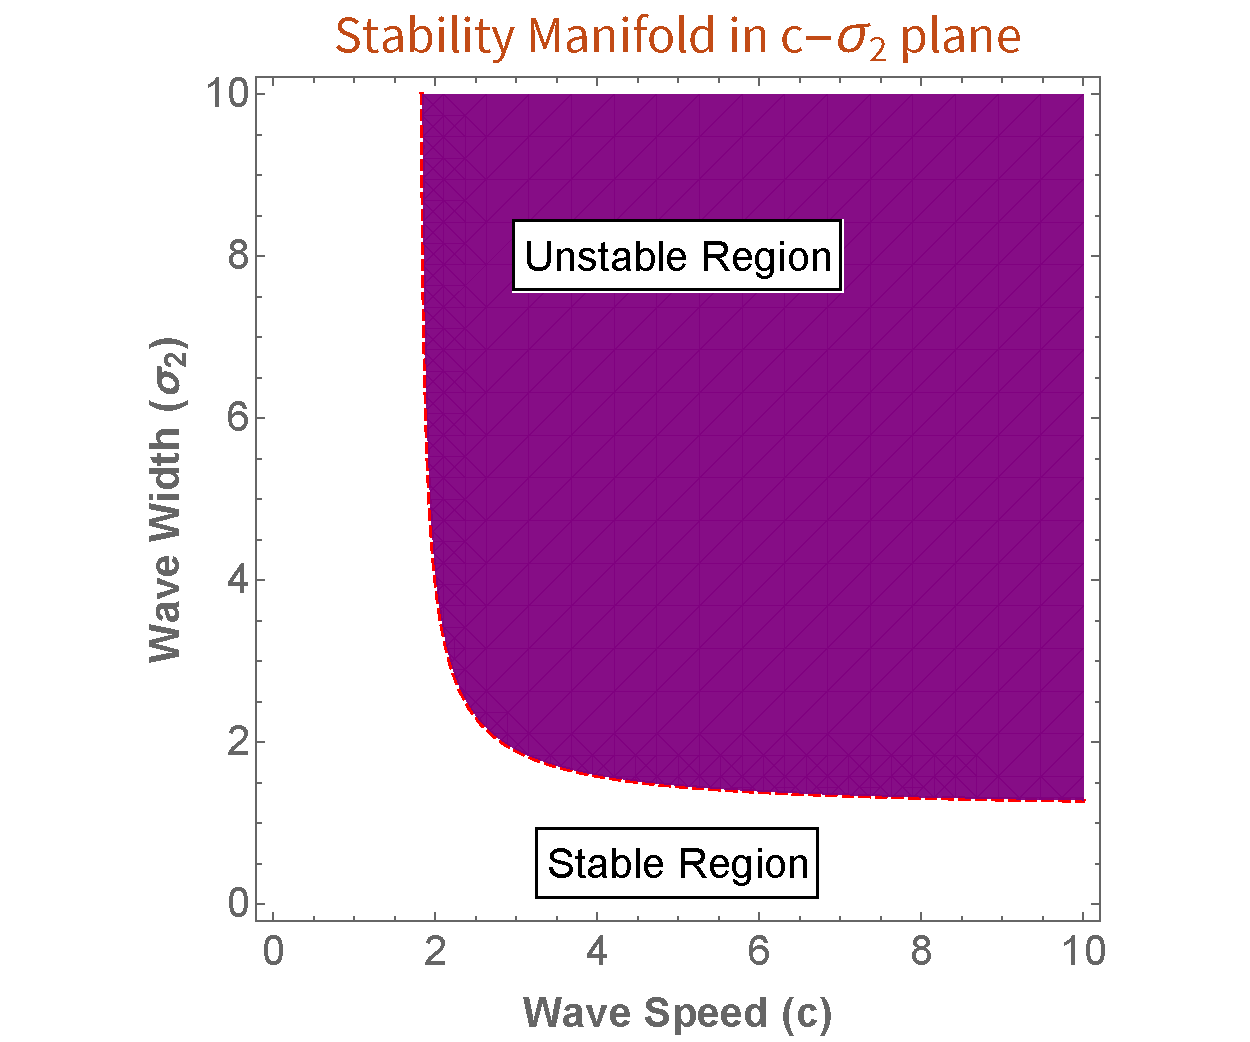
\includegraphics[width=0.75\textwidth]{images/nft_activity/stabilitysurface}
	\def\c{The manifold in $(c,\sigma_2)$ space which defines the stability of the final organisation. }
	\caption[\c]{\label{fig:stablity} \c Below the surface solutions do not exhibit singularities and the training function is deemed to be stable; in general, small choices for the parameters exhibit stable synaptic organisations at the cost of arbitrarily small amplitude. The manifold appears to be well-above reasonable estimates for these parameters, ensuring the model is likely stable in plausible biological scenarios.} 
\end{figure}
\paragraph{Fourier Space}
{  The Fourier transform of $S$ has a characteristic bump near the origin which decays to a constant representing a baseline level of noise  i.e. $\hat{S}(k) = c_0 + \hat{\mathcal{S}}(k)$ where $\hat{\mathcal{S}}(k)$ is a symmetric function decaying quickly to zero.} Note that it is possible for $\hat{\mathcal{S}}(k)$ to fall below the noise level which implies that the system will be out of phase and suppress signals at this wave length. A typical representation in Fourier and real space is shown in Figure \ref{fig:powerdistribution}a. 
\begin{figure}
	\centering
	\begin{subfigure}{0.4\textwidth}
		\centering
		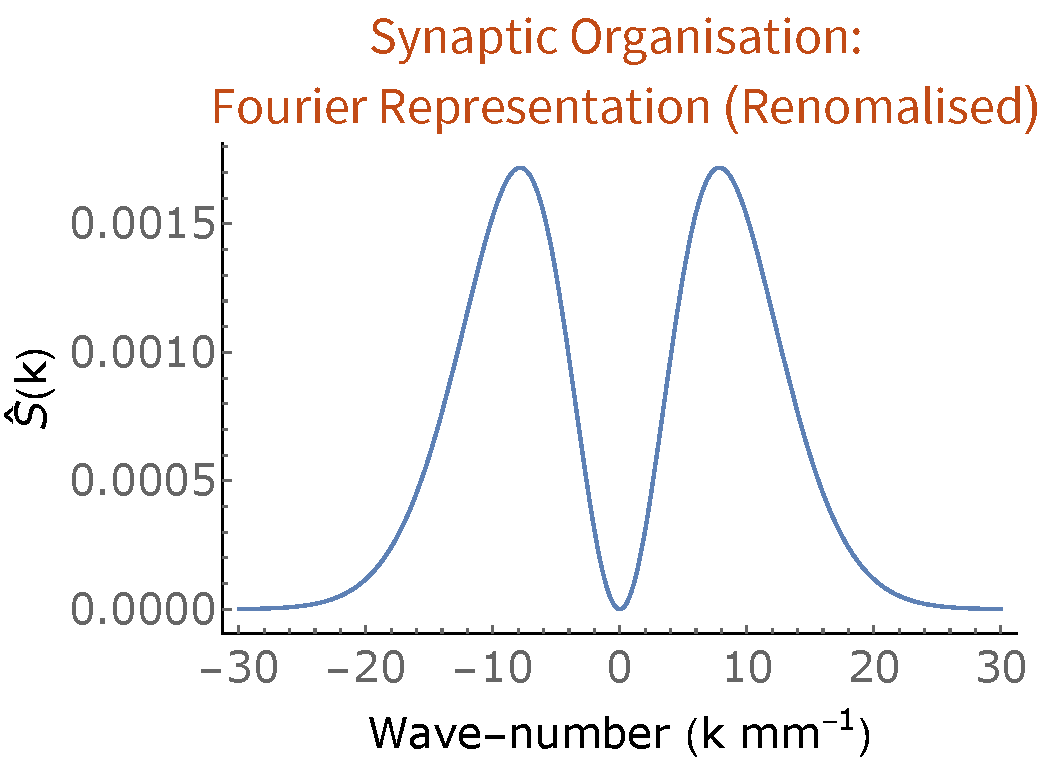
\includegraphics[width=\textwidth]{images/nft_activity/example-typicaldistributionfourier}
		\caption{}
	\end{subfigure}
	\begin{subfigure}{0.4\textwidth}
		\centering
		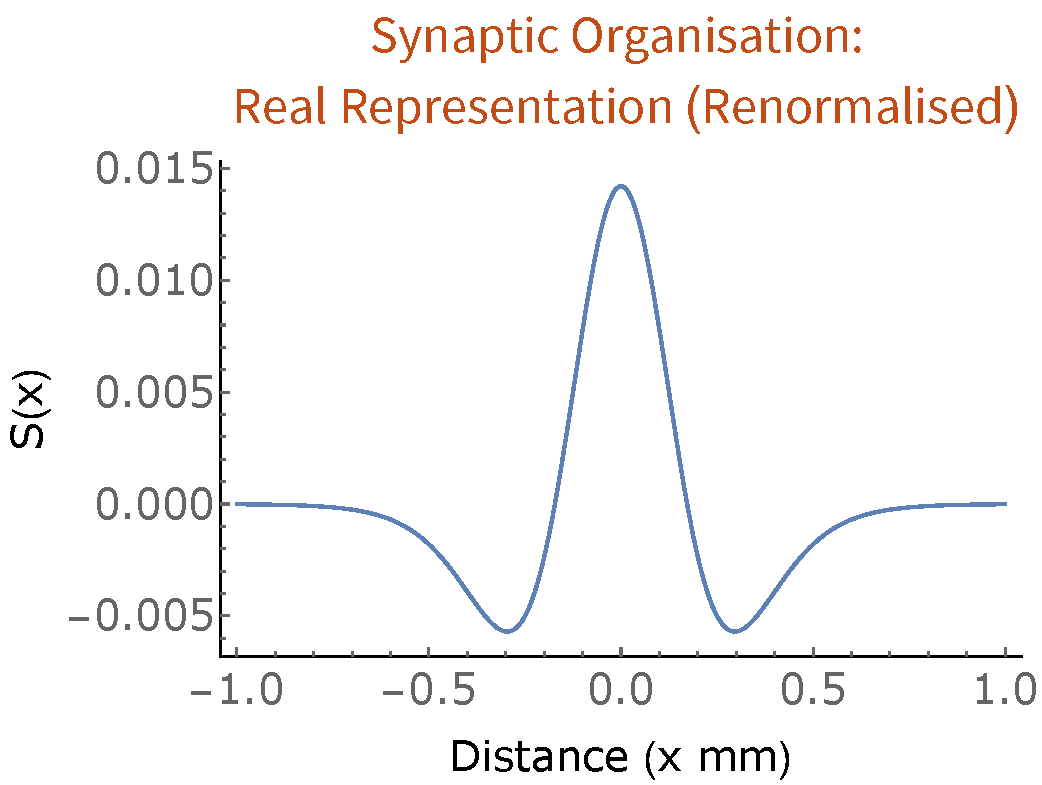
\includegraphics[width=\textwidth]{images/nft_activity/example-typicaldistributionreal}
		\caption{}
	\end{subfigure}
	\def\c{A typical organisation generated with the parameters shown in Table \ref{table:parameters} with (a) showing the representation in Fourier space, and (b) the representation in real space after re-normalisation. }
	\caption[\c]{\label{fig:powerdistribution} \c} 
\end{figure}

The distribution of the connections in physical space can be found by inverting its Fourier representation which presents a problem with the inclusion of the Dirac-Delta distribution introduced by $c_0$. This problem can be circumvented by realising that the baseline constant representation of all frequencies represents white noise which can be therefore be renormalised and omitted; see Figure \ref{fig:powerdistribution}b. This re-normalisation is done under the assumption that provided the amplitude of $\hat{\mathcal{S}}(k)$ provides a high enough signal-to-noise ratio then this system will be absorbed into already present biological noise which is filtered out in downstream calculations.
\paragraph{Refinement}
The steady state solution of the synaptic distribution $S$ takes its maximum at the origin and rapidly decays at large distances. The distributions feed-forward capability is therefore dictated by the magnitude at the origin and the rate of the decay. For precise signal transmission (or a refined retinotopy) the width of the distribution should be small with respect to the length scale. Width is estimated by taking the inverse of the wave-length that maximises the power spectrum:
\begin{equation} \label{eq:width}
	\Omega(\vec{\rho}) =  \frac{1}{\text{argmax}_k\left| \hat{S}(k;\vec{\rho})\right|},
\end{equation}
where $\vec{\rho}$ represents the vector of parameters which define the model. The width relationships in the plane of several pairs of variables within a stable region containing no singularities are examined and shown in Figure \ref{fig:parametereximinations}. Refinement tends to decrease in accordance with decreases in $c, \sigma_2, (r_1/r_2), R_1, t_p$, and $\tau$. On the biological scales of interest for the current work the decreases do not appear to be substantial in the $R_1$ and $\tau$ directions. In general the relationships between the variables are non-linear.

\begin{figure*}[h!]
	\centering
	\begin{subfigure}{0.45\textwidth}
		\centering
		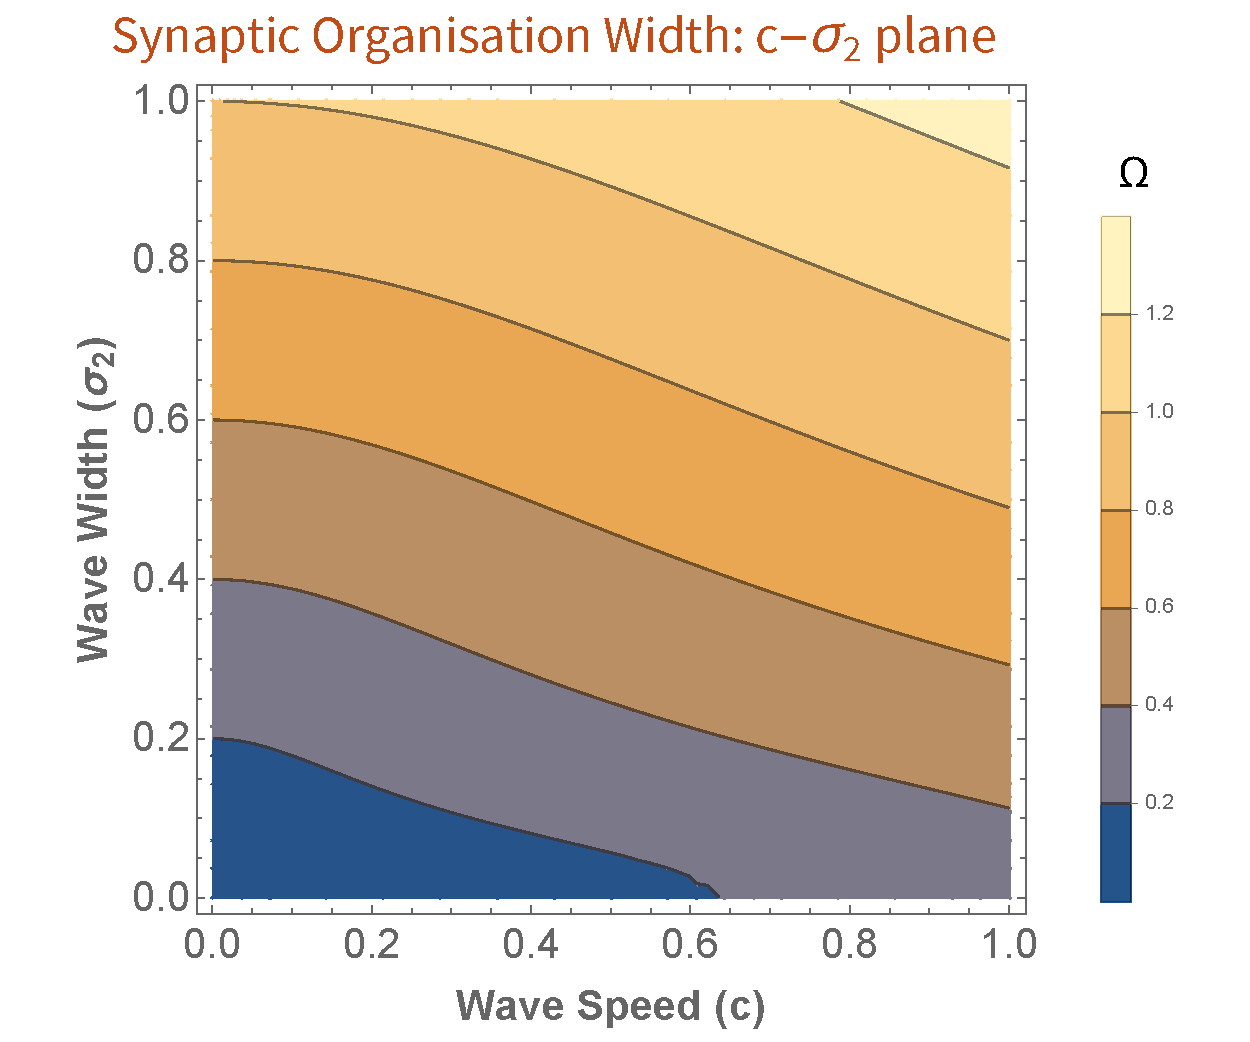
\includegraphics[width=\textwidth]{images/nft_activity/width_cs2}
		\caption{}
	\end{subfigure}
	\begin{subfigure}{0.45\textwidth}
		\centering
		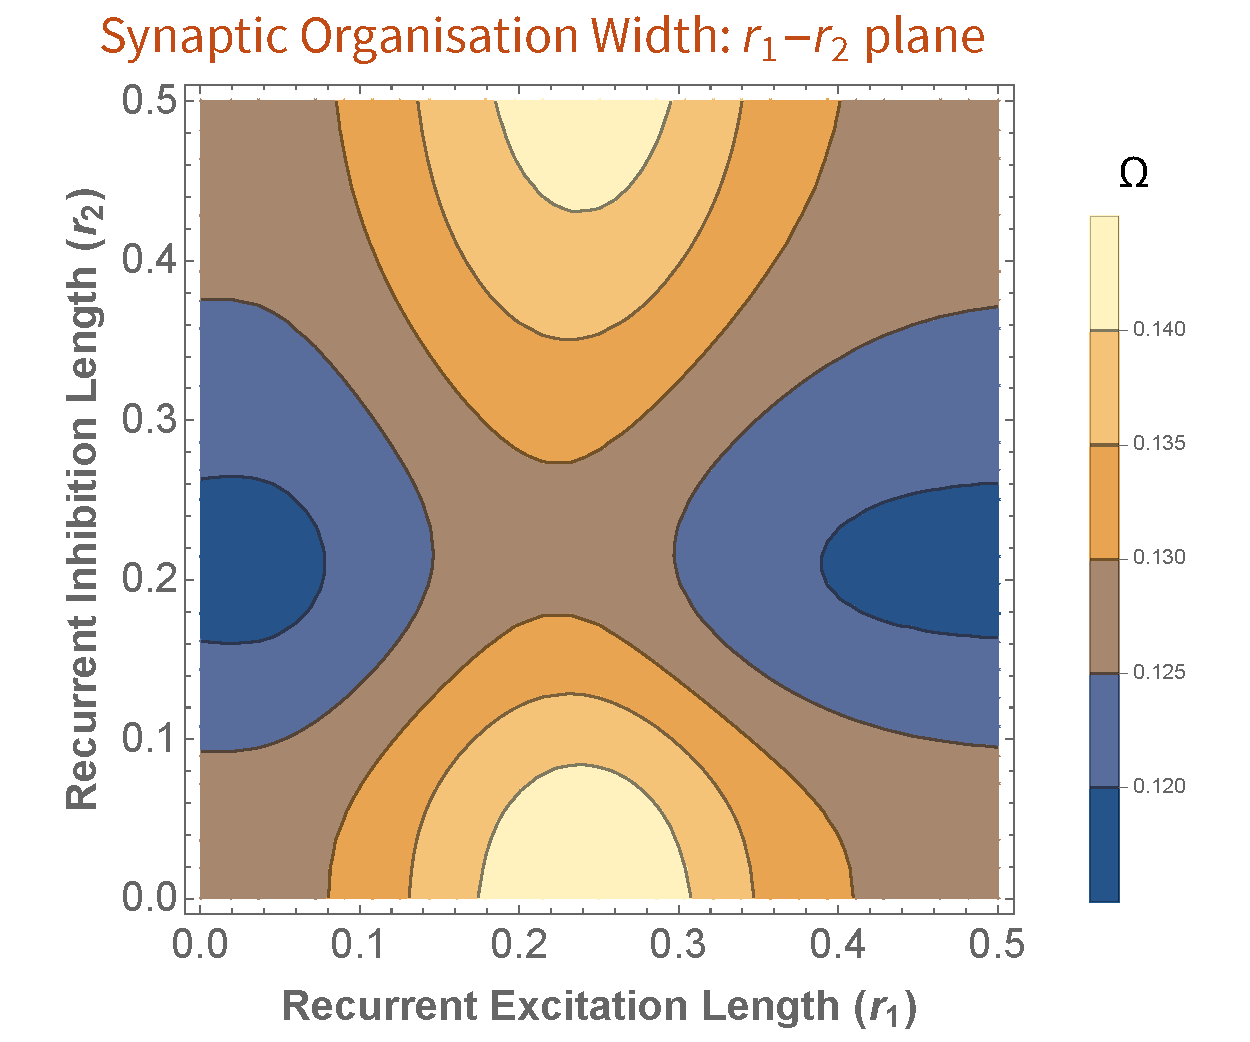
\includegraphics[width=\textwidth]{images/nft_activity/width_r1r2}
		\caption{}
	\end{subfigure}
	\begin{subfigure}{0.45\textwidth}
		\centering
		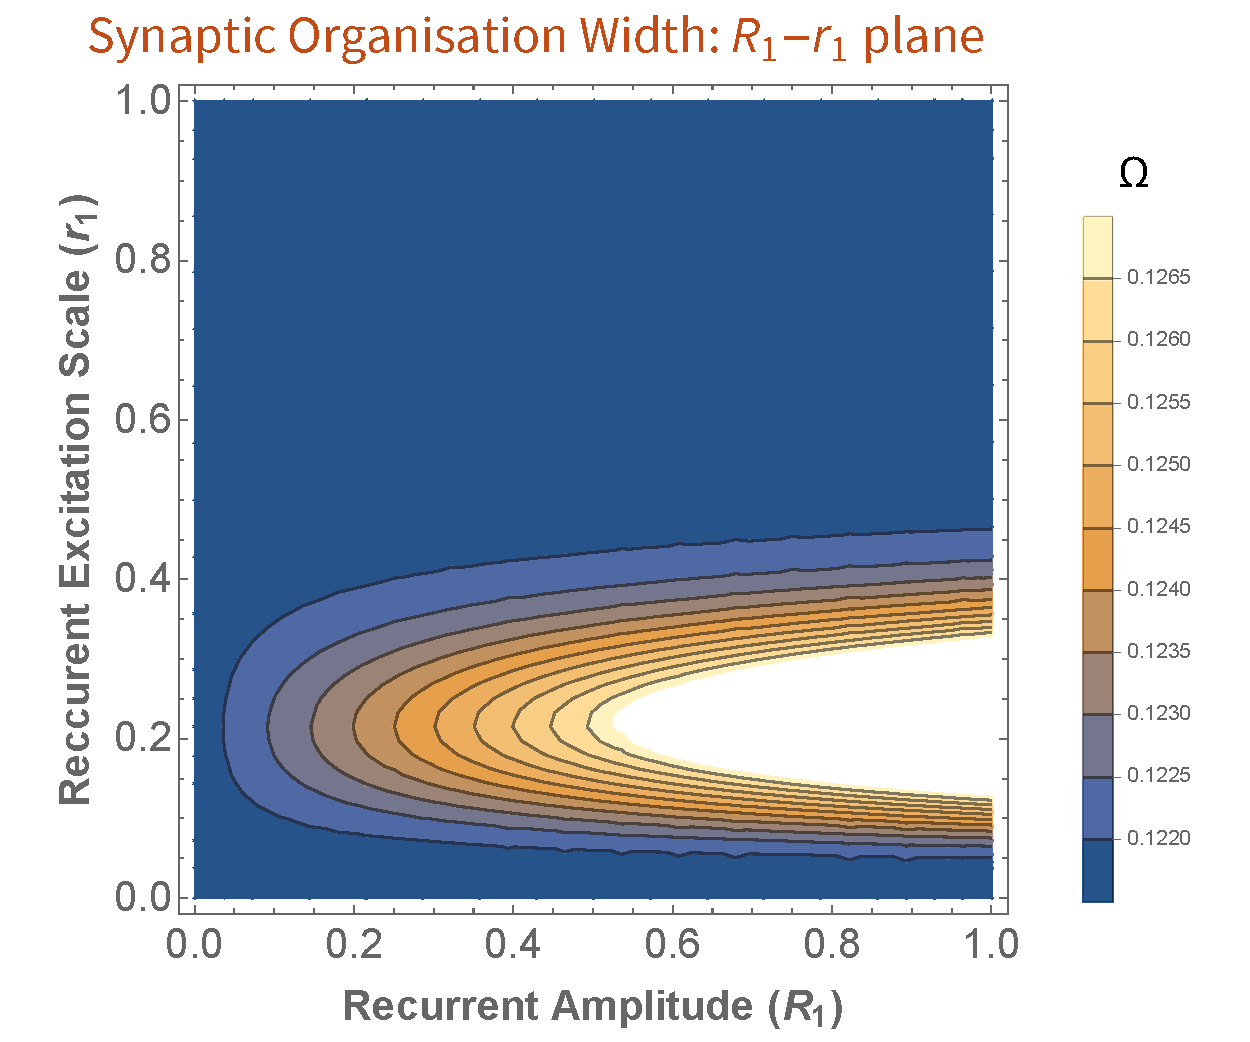
\includegraphics[width=\textwidth]{images/nft_activity/width_R1r1}
		\caption{}
	\end{subfigure}
	\begin{subfigure}{0.45\textwidth}
		\centering
		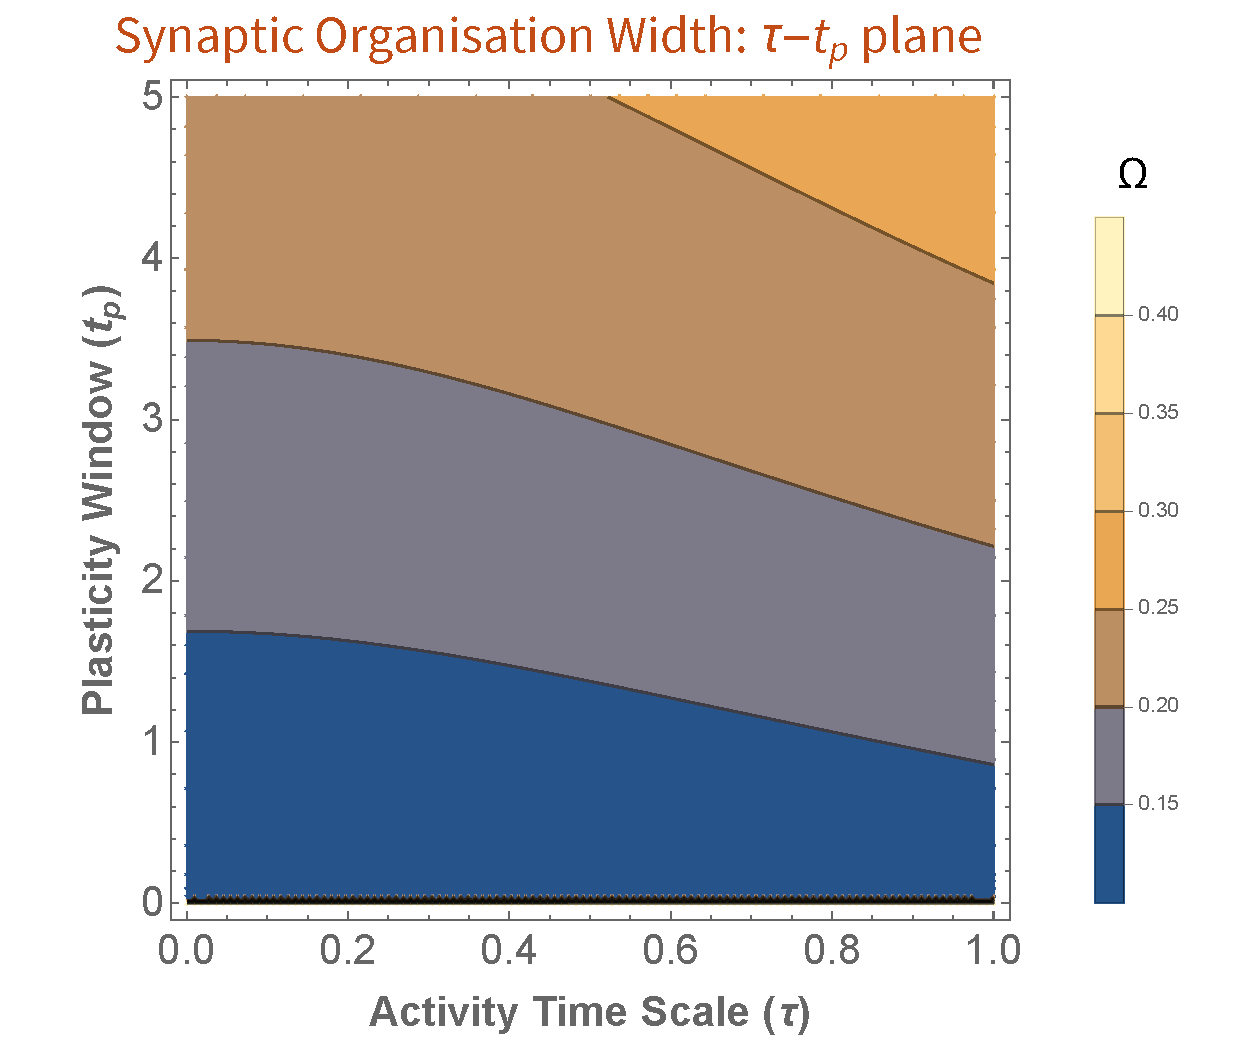
\includegraphics[width=\textwidth]{images/nft_activity/width_tautp}
		\caption{}
	\end{subfigure}
	\def\c{The variation in width ($\Omega$) in four distinct planar slices of the manifold of parameters which influence the models prediction of mean distribution width. }
	\caption[\c]{\label{fig:parametereximinations} \c Panel (a) shows that width decreases both with wave-speed and wave-width, qualitatively accounting for the differences between the wild-type and $\beta2^{-/-}$ mutant. Panel (b) shows that width decreases with with the ratio of excitation to inhibition in the recurrent connections $W$ suggesting a smaller zone of excitatory support decreases arbor size. There is an anti-symmetry along the line $r_1 = r_2$ which is expected as the dominant connection type switches along this line.  Panel (c) shows that width decreases with recurrent connection amplitude but the effect is not substantial. Panel (d) shows that width predominately decreases in accordance with the plasticity window time-scale, and while the activity time-scale has an effect it is not substantial.}
\end{figure*}

\paragraph{Sensitivity}
{ In the context of refinement it is prescient to consider which parameters affect the models prediction of the width $\Omega$ in equation \ref{eq:width}. This width will satisfy $dS(k; \vec{p})/dk = 0$ which inserted into equation (\ref{eq:asymptoticsynapse}) yields:}
\begin{equation}
	\frac{dg(k; \vec{p_g})}{dk} = 0,
\end{equation}
where $\vec{p_g} = \{c, \tau, t_p, \sigma_2, R_1, r_1, r_2\}$. The width will only vary in accordance with these parameters which is confirmed by numerical simulation.


\paragraph{MCMC Parameter Estimation}
The $\beta2$ knock-out in mouse has the effect of broadening the spatio-temporal patterns of spontaneous activity in the retina and SC during development \cite{ Stafford2009}. The mutant mice have substantially wider arborisations than in wild-type establishing the importance of activity in refining the retinotopic projection \cite{Dhande2011-jp}. Existing models have not been able to predict this wider arborisation when the patterns of activity associated with the knock-out are replicated in the model's mechanisms for activity \cite{Lyngholm2019-fs}.

\begin{figure*}[h!]
	\centering
	\begin{subfigure}{0.475\textwidth}
		\centering
		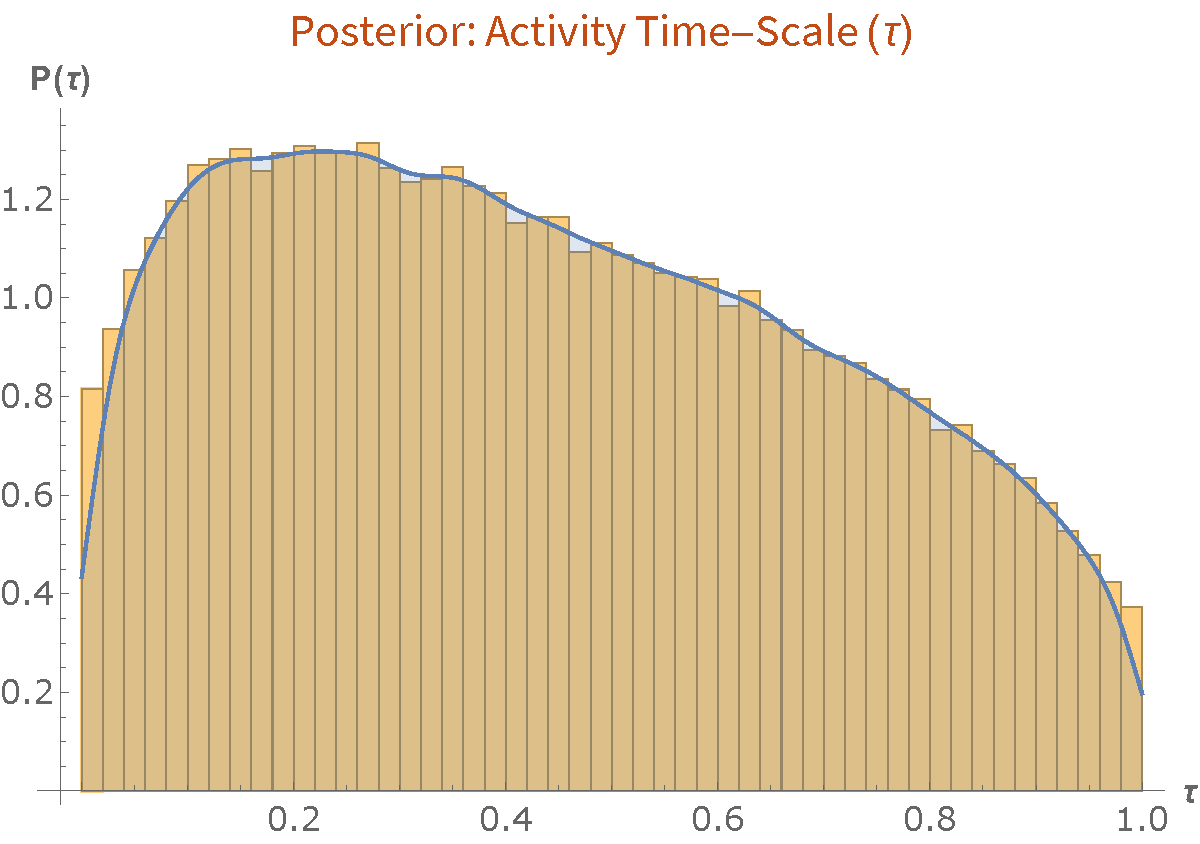
\includegraphics[width=\textwidth]{images/nft_activity/posterior_tau}
		\caption{}
	\end{subfigure}
	\begin{subfigure}{0.475\textwidth}
		\centering
		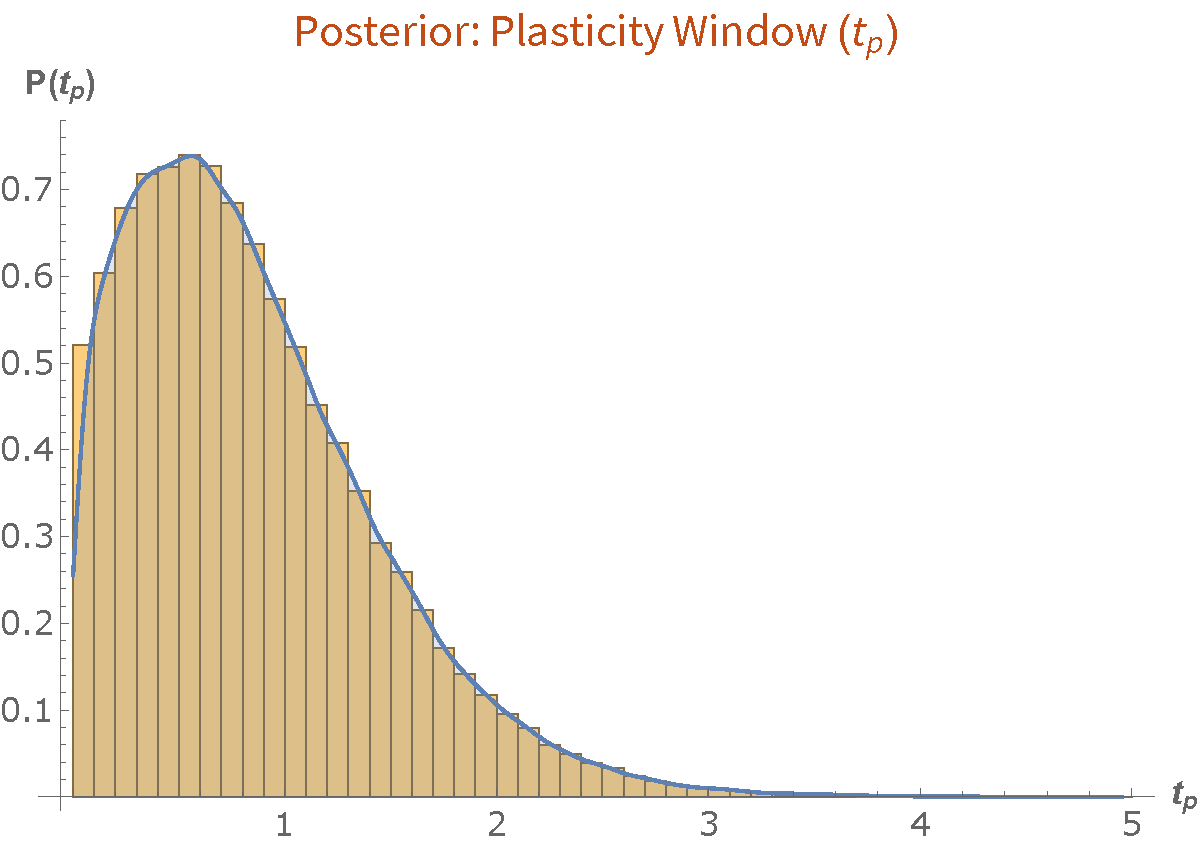
\includegraphics[width=\textwidth]{images/nft_activity/posterior_tp}
		\caption{}
	\end{subfigure}
	\begin{subfigure}{0.475\textwidth}
		\centering
		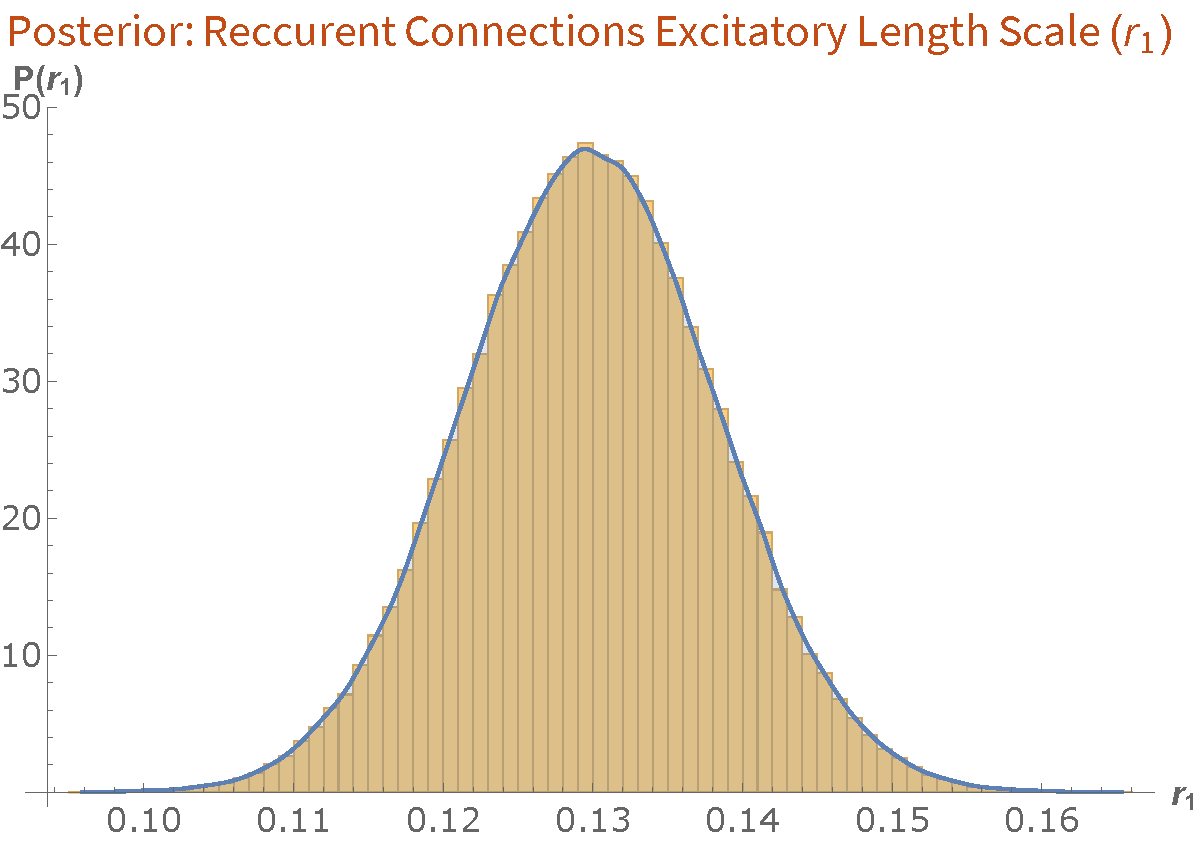
\includegraphics[width=\textwidth]{images/nft_activity/posterior_r1}
		\caption{}
	\end{subfigure}
	\begin{subfigure}{0.475\textwidth}
		\centering
		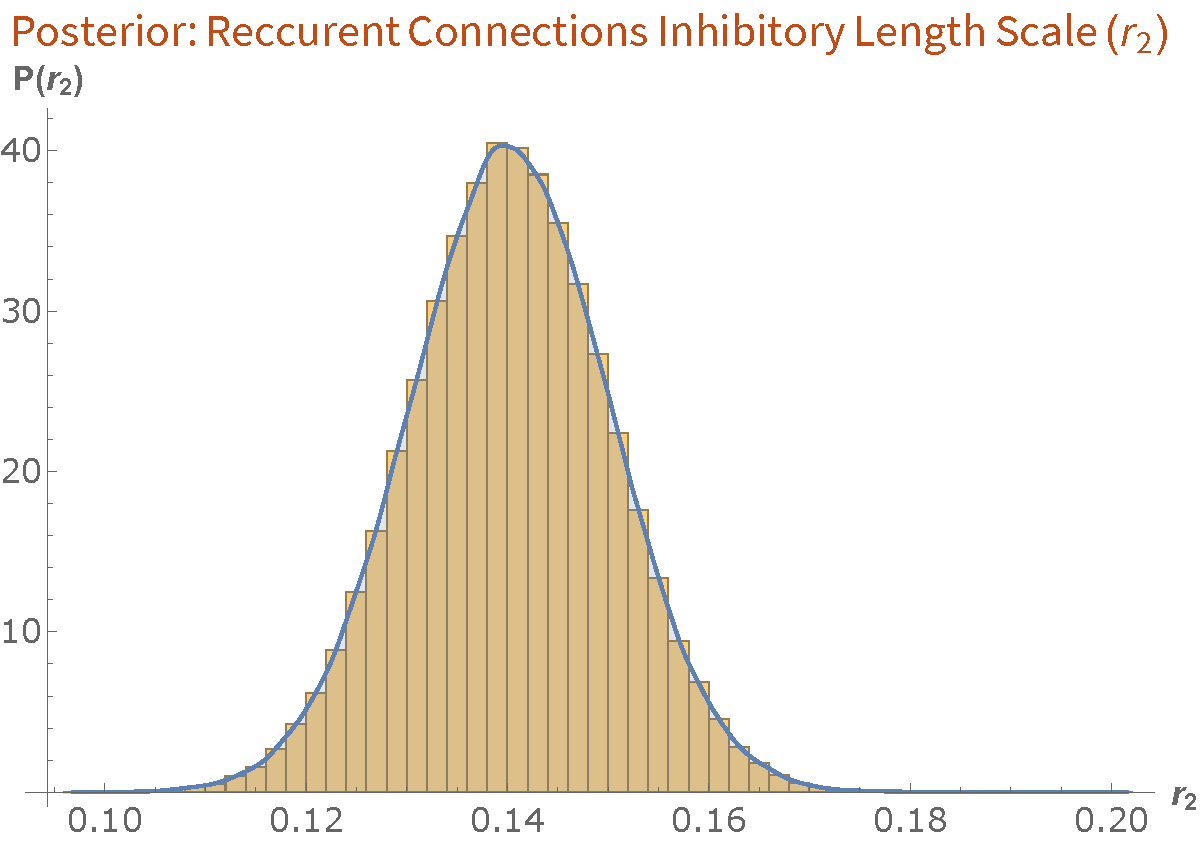
\includegraphics[width=\textwidth]{images/nft_activity/posterior_r2}
		\caption{}
	\end{subfigure}
	\begin{subfigure}{0.475\textwidth}
		\centering
		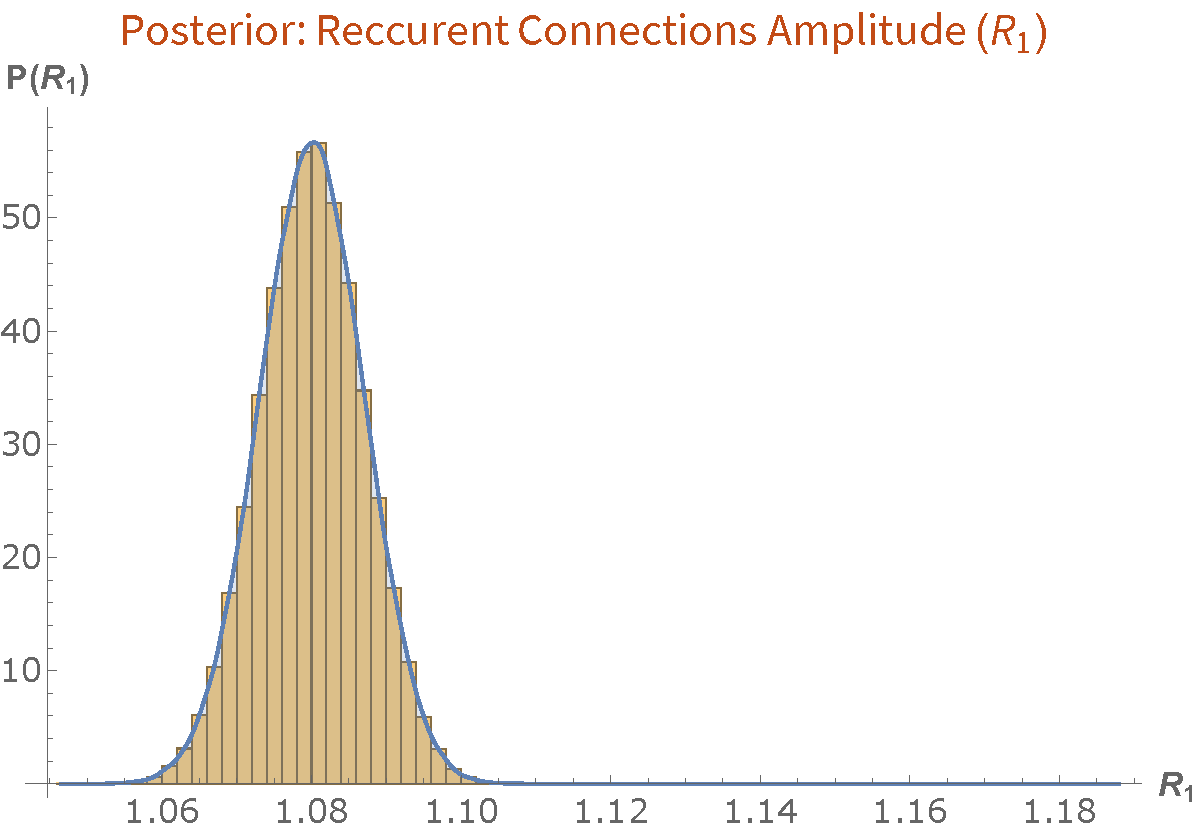
\includegraphics[width=\textwidth]{images/nft_activity/posterior_R1amp}
		\caption{}
	\end{subfigure}
	\def\c{The posteriors for the relevant model parameters after an MCMC regression. }
	\caption[\c]{\label{fig:posteriors} Panel (a) shows the posterior histogram for the time-scale of activity which is broadly distributed through the search space of [0,1]s but biased towards the lower bound. This broad distribution is concordant with the observation that the time-scale of activity induces relatively small variations in the organisation width; see Figure \ref{fig:parametereximinations}. Panel (b) shows the posterior histogram for the time scale of the plasticity window which is maximised around 0.6s. The posterior histograms for the recurrent connection parameters $(r1, r2, R1)$ are shown in Panels (c-e) and are tightly constrained by their informative priors suggesting that there is no predicted effect on these connections in the $\beta2^{-/-}$ mutant. For all histograms presented an empirical distribution curve was fitted and overlain in blue.}
\end{figure*}
The arborisation widths are estimated as $0.24 \pm 0.077 \text{mm}$ (wild-type) and $0.48 \pm 0.15 \text{mm}$ ($\beta2^{-/-}$) by taking half the square root of the arborisation area reported by Dhande et. al. (2011) \cite{Dhande2011-jp}. The wave speeds are estimated as $0.13 \pm 0.015 \text{mm s}^{-1}$ (wild-type) and $0.17 \pm  0.03 \text{mm s}^{-1}$ ($\beta2^{-/-}$), and the wave-widths as $0.11 \pm 0.012 \text{mm}$ (wild-type) and $0.20 \pm 0.012 \text{mm}$ ($\beta2^{-/-}$) by taking half the total width reported by Stafford et al (2009) \cite{Stafford2009}. The inhibitory and excitatory lengths scales, and amplitude of the recurrent connections are estimated as $0.14 \pm 0.014 \text{mm}$ and $0.13 \pm 0.013 \text{mm}$, and $1.08 \pm 0.01 \text{mm}$ respectively using the data reported by \cite{Phongphanphanee2014-in}. The priors on these parameters are taken as normal distributions centred on the estimates with standard deviation corresponding to the measurement error. Uninformative priors on the time-scale parameters are taken assigning uniform distributions on [0,1] and [0,10] for the activity time scale ($\tau$) and the plasticity window scale ($t_p$), respectively. The MCMC was completed using a dedicated Mathematica package \cite{Burkart2017}. The MCMC completed in $10^5$ iterations using 6 chains with each parameter initialised within 10\% of the mean of its prior. The maximum Gelman-Rubin statistic for convergence was $1.00037$ indicating that the chains had converged \cite{Gelman1992-pk}. The posteriors for each parameter are reported in Figure \ref{fig:posteriors}. The posteriors for the recurrent connections parameters, $r1, r2$, and $R_1$ remained tightly constrained by their priors, indicating that the prior estimates were well informed and in agreement with the model. The activity time scale is broadly distributed throughout the range [0,1]s with a bias towards 0. The plasticity time-scale is distributed around a maximum of $0.56$s. The computed $R^2$ statistic was 0.81. The code base for these simulations is freely available online \cite{NFT}.
\section{Discussion}
If the model is sound and the biological system is allowed sufficient time to reach a reasonable approximation of the asymptotic state then these results suggest that the computational/synaptic structures developed are primarily a result of activity dynamics. Under this model the chemotactic and competitive mechanisms serve to initialise a coarse isotropic retinotopy from which the activity dynamics can refine and ultimately dictate final synaptic organisation. This interpretation augments the understanding of the establishment of retinotopy by suggesting that the final synaptic organisation can be understood in a large part by understanding the spatio-temporal nature of the input stimulus, the recurrent connectivity, and the learning rule. Should the biological system not employ the learning routine until asymptotic stability then the model will still be able to make predictions about the final organisation given precise enough measurements of the relevant parameters. In both instances the model gives testable hypotheses the former of which has been benchmarked against the mouse wild-type and $\beta2^{-/-}$ mutant.

\paragraph{Organisation}
The key aspects of the final organisational structure are dictated by the interplay between the spatio-temporal characteristics of the input stimulus and the structure of the recurrent connections. These dependencies on recurrent connections and input are in accordance with previous analysis performed with a simple Hebbian rule and static input \cite{Takeuchi1979-zy}; the model proposed here, however, allows for richer construction in terms of specifying the input and connections by realising full temporal and spatial dynamics, and more complex structure in the final organisation. Regularisation rules were introduced which allow this organisation to take non-trivial structure when supplemented by system noise which is assumed able to be renormalised in downstream biological calculations or via some other mechanism. The regularisation necessitates neurotrophic factors being expressed during development. Finally, the measurable aspects of the organisation are dictated by the precise realisation of the relevant biological parameters.
\paragraph{Refinement}
The results indicate parameter dependence on wave-speed, wave-width, plasticity time-scales, and the ratio of excitation to inhibition widths in the recurrent connections. Principally, parameter changes that would lead to a tighter correlation structure such as smaller wave-widths, slower wave-speeds, and smaller excitatory zones lead to a smaller width of topographic refinement. Interestingly, the time-scale of the plasticity rule has an effect of the width of the final organisation. The $\beta2^{-/-}$ mutant provides a phenomenological test of this component of model. The knock-out exhibits fast-moving, and hyper-correlated, retinal waves which lead to an imprecise topographic mapping - an effect that has not been captured in existing models. The model suggests that an increase in wave-speed or wave width will lead to a less-refined map reproducing the results of the knock-out \textit{in silico}; see Figure \ref{fig:parametereximinations}. 

An MCMC parameter estimation was performed using known errors-in-measurement of wave-speed, wave-width, and organisation width in wild-type and the $\beta2^{-/-}$ mutant. The model predicts the expected mean width of both wild-type and the $\beta2^{-/-}$ mutant within standard error when parametrized by likelihood maximising parameters and provides a good explanation of the variance between the wild-type and mutant ($R^2$ = $0.81$).  The model is insensitive to the time-scale of activity with the posterior assuming a broad posterior over $[0,1]$s with a slight bias towards lower values suggesting that the activity time-scale does not account for much of the variance in organisation width. The posteriors of the parameters of the recurrent connections were largely dictated by their priors suggesting that the priors estimated from available are informative and that the $\beta2^{-/-}$ mutant does not have a substantial effect on the recurrent connections, as expected. The time-scale of the plasticity window is not expected to be affected by the knock-out and thus the MCMC allows us to estimate this parameter on the order of seconds. { The timescale of the plasticity window in two closely related biological systems, the Xenopus retinotectal projection and rat visual cortex, are estimated to be on the order of $10^{-2}$ seconds \cite{Froemke2002-be, Zhang2000-lb}. Plasticity windows can have significantly longer time-scales on the order of 10s of minutes \cite{Citri2008-kv}. The estimate is notably higher than what has been observed in similar systems but is in agreement with the typical duration of a wave of spontaneous activity in the developing retina in mice \cite{Xu2015-uc}. Deviation is expected in analysing a different biological system. This result suggests that the plasticity windows in this system are calibrated to integrate all information contained in a spontaneous wave event.}
\paragraph{Limitations}
The model presented here has several key limitations: dimensionality,  stimulus representation, simplicity of asymptotic solution, non-rigorous estimate of recurrent connectivity. The model is one dimensional while the surface of the superior colliculus is a two dimensional sheet. Two dimensional systems allow for a much richer topology and complicated dynamics which would be best examined numerically. The stimulus was assumed to be a simple wave-packet travelling left or right at a fixed speed and these directions were assumed to be equiprobable. These assumptions do not hold in two dimensional recordings with a directional bias being observed in retinal waves in mouse \cite{Ackman2012-uu}. The assumptions allowed an analytical solution to be derived which assisted with the MCMC simulations but is valid only asymptotically. The biological system has fixed developmental time frames and critical periods. Finally, the recurrent connections are assumed to be the difference of two Gaussian's with parameters estimated from a fit made to electrophysiological recordings \cite{Phongphanphanee2014-in}. This assumption is reasonable but would require extensive validation and a more rigorous biological underpinning would be desirable.
\paragraph{Future Directions}
The limitations listed above outline a clear direction for future study: extensive numerical simulation in a two dimensional context. The analysis can be trivially extended into the plane by using the same assumption: every wave-direction is equiprobable. A more realistic simulation can be conducted using data from a repository of retinal waves or by generating synthetic data from a wave-model \cite{Eglen2014-fo, Godfrey2009-rs}. A challenging aspect of this line is computational cost: the analytical solution is cheap to evaluate but numerics will take substantially longer. A method of mitigating this is by using GPU architectures and exploiting the parallelisation benefits of matrix multiplication which is required to evaluate the convolutional integrals. GPU parallelisation will be used in following chapters for similar reasons. This can be complemented with solvers developed for the Julia computing language which offer good numerical performance \cite{Sequeira2022}.

The model predicts that the time-scale of the plasticity window in developing mouse SC neurons is an order of magnitude higher than the scale typically used to describe neuronal plasticity in analogous systems. This prediction is not claimed to represent a ground truth, the model makes several simplifying assumptions and estimations, but it is a good candidate for experimental falsification.
\paragraph{Key Summary}

\begin{enumerate}
	\item \textit{An NFT modelling framework has been developed to allow for the incorporation of complex spatial statistics of retinal waves. Within this framework an analytical solution for plausible input stimulus was derived allowing for efficient computation.}
	\item \textit{Bayesian statistical regression showed the model can explain existing wild-type and mutant data. The regression also made a falsifiable experimental prediction about the time-scale of plasticity estimating it at ~0.5 a second in mice.}
	\item \textit{The model is naturally extendable to two dimensions and allows for efficient numerical simulation of realistic biological wave statistics.}
\end{enumerate}